\section{Magnetometr}
Jednym z elementów większości Inercjalnych Systemów Nawigacyjnych jest
magnetometr. Wykorzystoje się go do określenia kierunku w którym porusza się dane
ciało. Typów czujników mierzących pole magnetyczne jest wiele. Do tego
zastosowaniu istotny jest jedynie pomiar indukcji pola magnetycznego ziemi która
wynosi od $30\mu T$ do $60\mu T$.
\\

\begin{figure}[!ht]
 \centering
 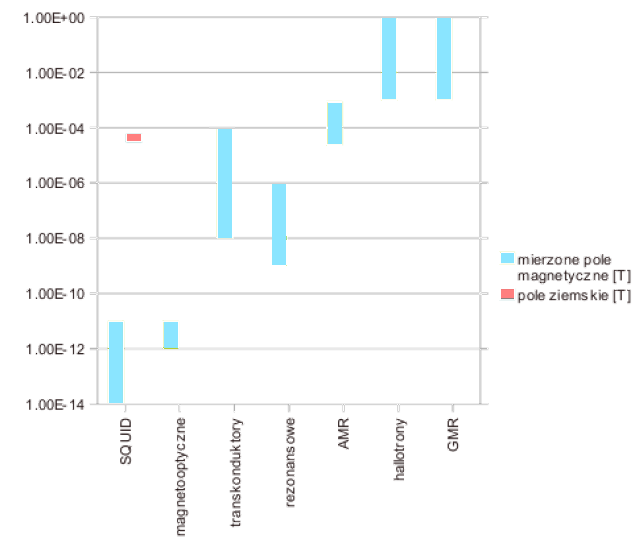
\includegraphics[height=100mm]{../images/ch04/magnetic_sens_types.png}
 \caption{Zakresy czujników pola magnetycznego różnego typu \cite{WstepnyProjektModuluIMU}}
 \label{fig:WykresMagnet}
\end{figure}

Na rysunku \ref{fig:WykresMagnet} przedstawione są zakresy pomiarowe czujników
pola magnetycznego różnego typu. Jak widać tylko dwa rodzaje magnetometrów z
wyżej wymienionych posiadają zakres pokrywający zakres indukcji pola
magnetycznego ziemi. Są to magnetometry transduktorowe oraz AMR\footnote{AMR - }.
% http://www.iemw.tuwien.ac.at/publication/workshop0600/Hauser.html